\documentclass[twocolumn,11pt]{abst}





% タイトル
\title{マルチコプターの高度制御}%高度制御を利用して自動着陸する研究}

\author{又村峰裕(指導教員 伊藤恒平)}

%\urlstyle{rm}

\setcounter{page}{9}
\lhead{}
\chead{}
\rhead{{\sf 18・204}\\{\bf 機械工学科}}
\lfoot{}
%\cfoot{{\sf-\ M-\thepage \ -}}
\cfoot{
 \ifnum \value{page} < 10
  {\sf-\ M-07}%\thepage \ -}
 \else%
  {\sf-\ M-08}%\thepage \ -}
 \fi%
}
\rfoot{}
\renewcommand{\headrulewidth}{3pt}
%\renewcommand{\footrulewidth}{1pt}



\begin{document}
%\layout
\maketitle
\thispagestyle{fancy}
\pagestyle{fancy}

\setlength{\baselineskip}{5.6truemm}
\kanjiskip=.07zw plus 3pt minus 3pt
\xkanjiskip=.07zw plus 3pt minus 3pt


% 本文

\section{はじめに}
\subsection{研究の背景}
ドローンとは,無人で遠隔操作や自動制御によって飛行できる航空機の総称のことである.ドローンの始まりは軍事用に偵察や攻撃用が作られた事が始まりである.近年,宅配サービスや農薬を撒く農業用,空撮,水中撮影,掌に収まるくらいの小型用,娯楽等のドローンが普及してきた.3つ以上のメインローターを持つヘリコプターをマルチコプターと呼び,その中から4つのメインローターを持つクアッドコプター(図1)について研究する.室内で使うことのできるマルチコプターは多くない.%(図\ref{fig:ensyu3tex})について研究する.室内で使うことのできるマルチコプターはあまり多くない.

\begin{figure}[htbp]
  \begin{center}
   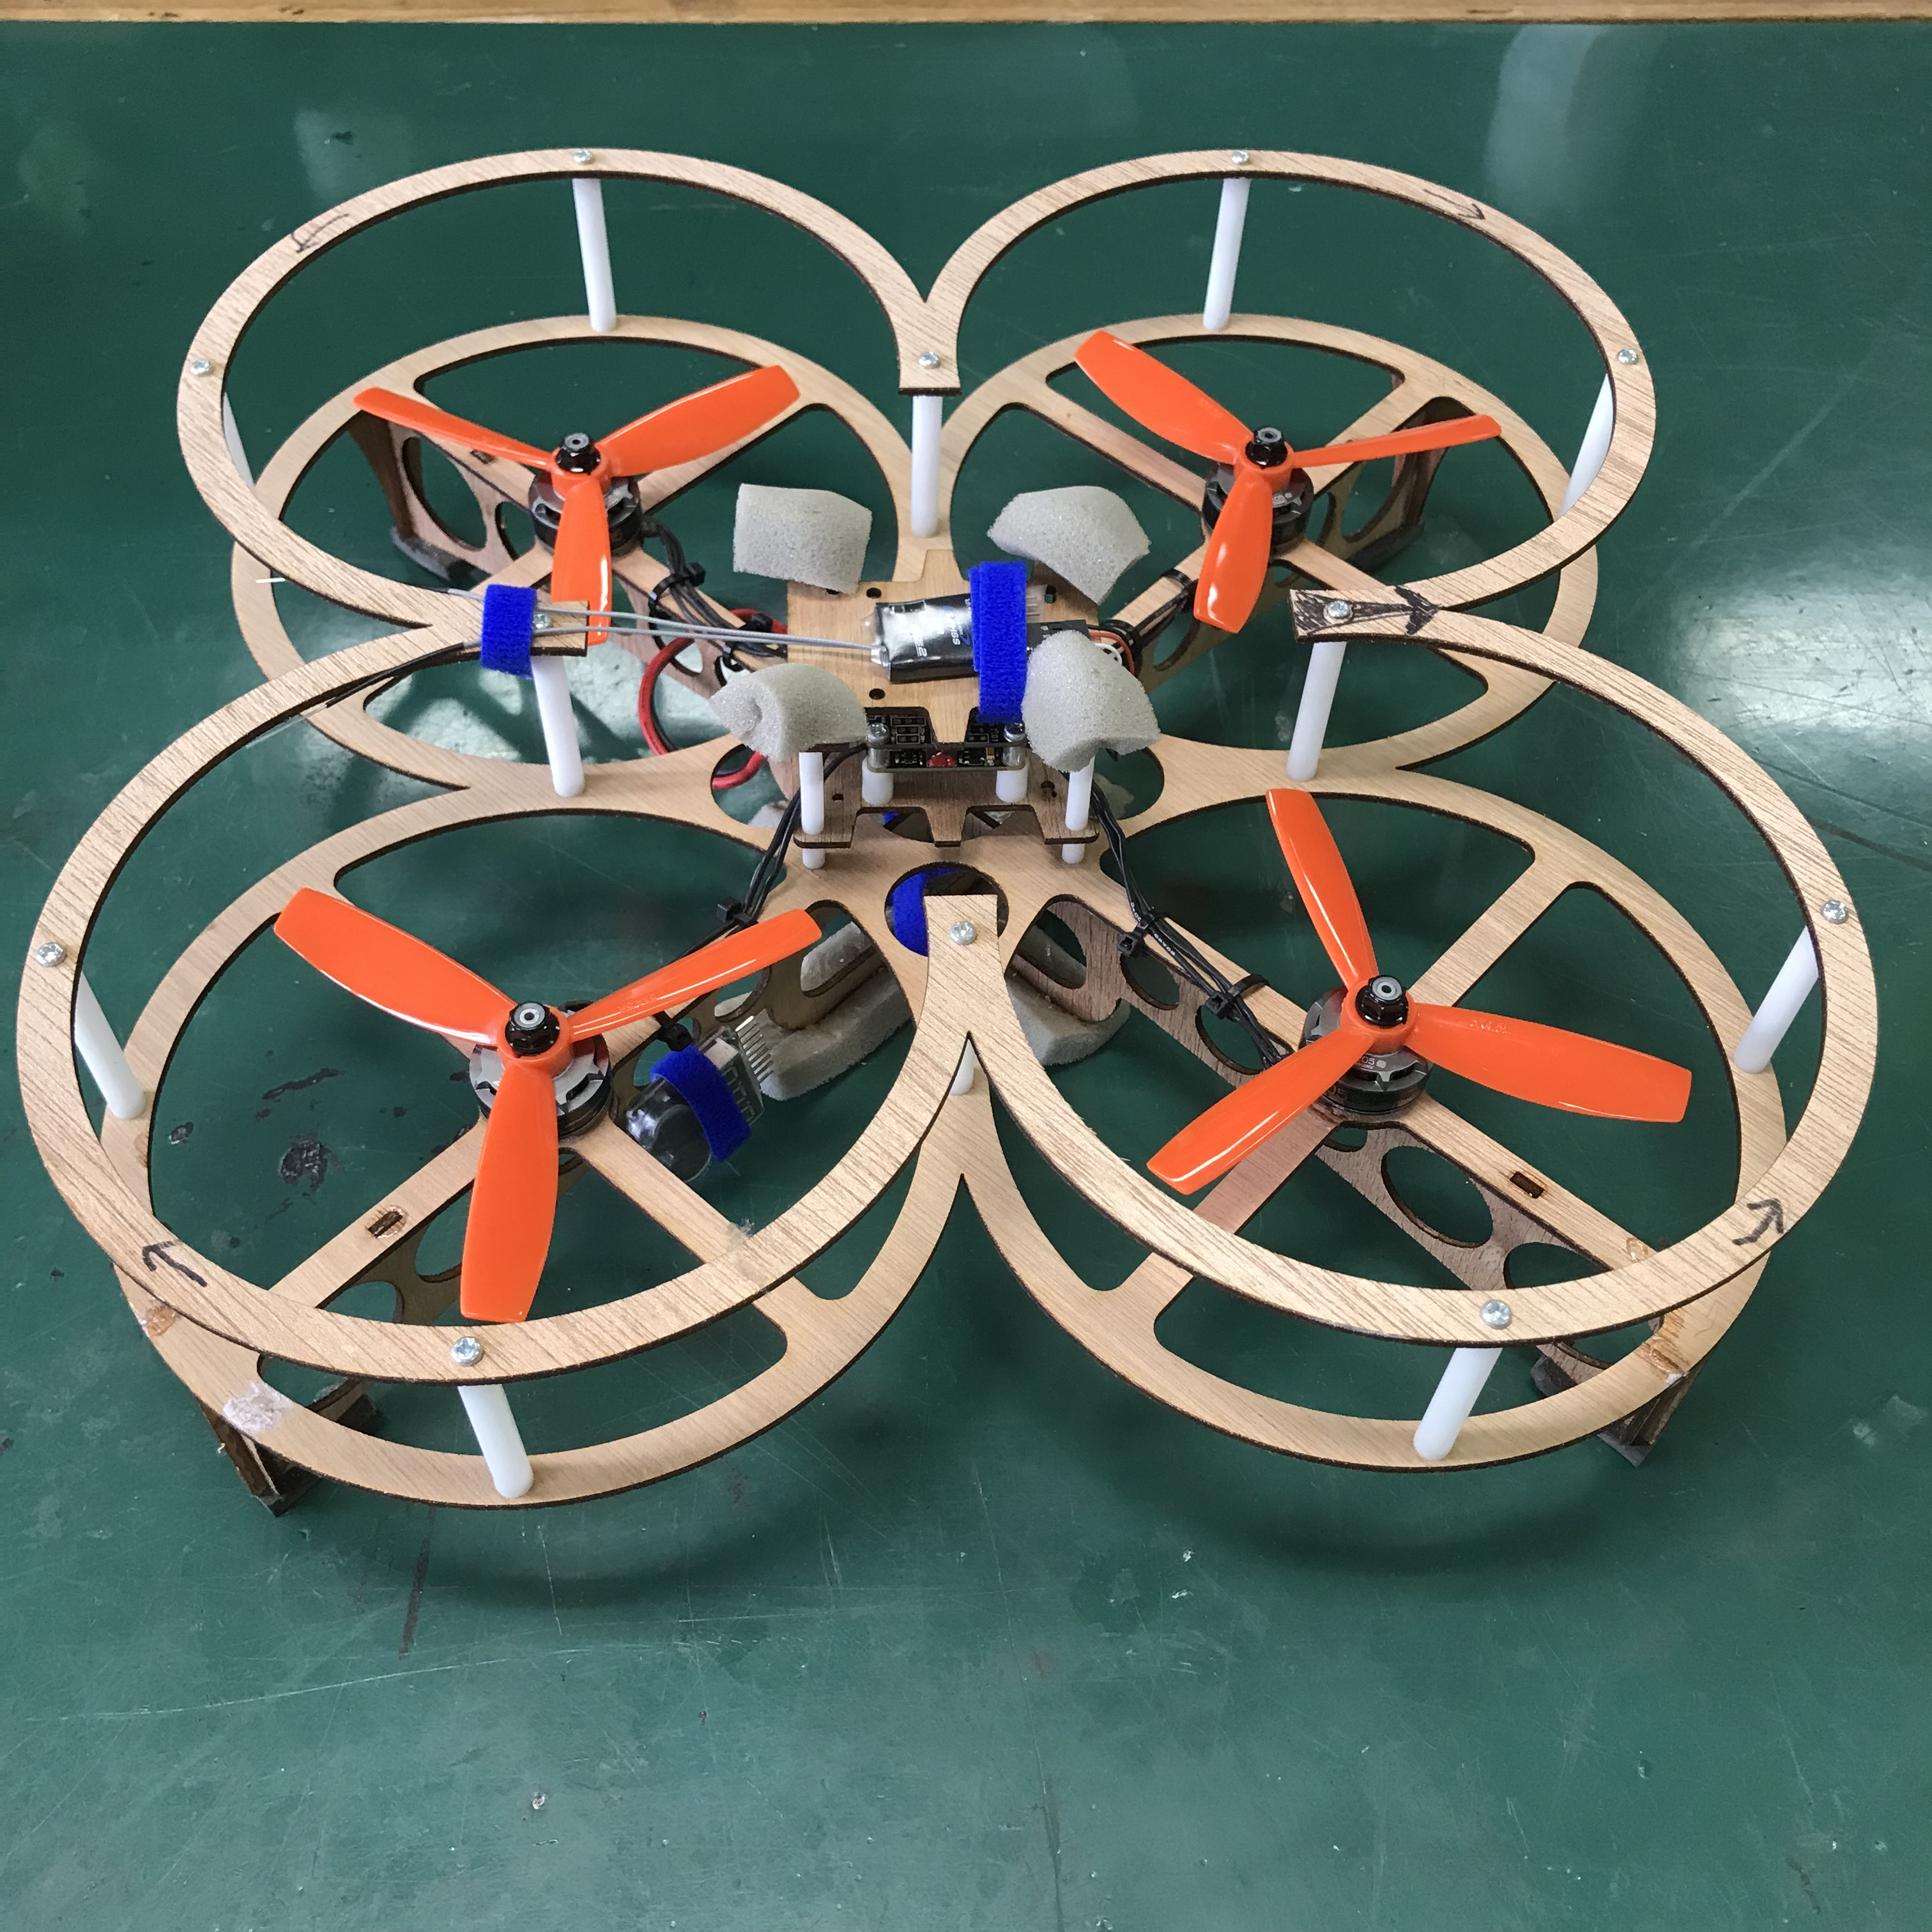
\includegraphics[width=30mm]{img/drone.jpeg}
    \end{center}
  \caption{クアッドコプター}
 \label{fig:ensyu3tex}
\end{figure}

%※初期drone図を入れる

中間目標の全日本学生室内飛行ロボットコンテストに図2に示すマルチコプターで出場しすべてのミッションに成功し,11チーム参加する中で優勝した.そこで挑まなかったミッションの中に自動制御があった.%(図\ref{fig:ensyu3tex})

\begin{figure}[htbp]
  \begin{center}
   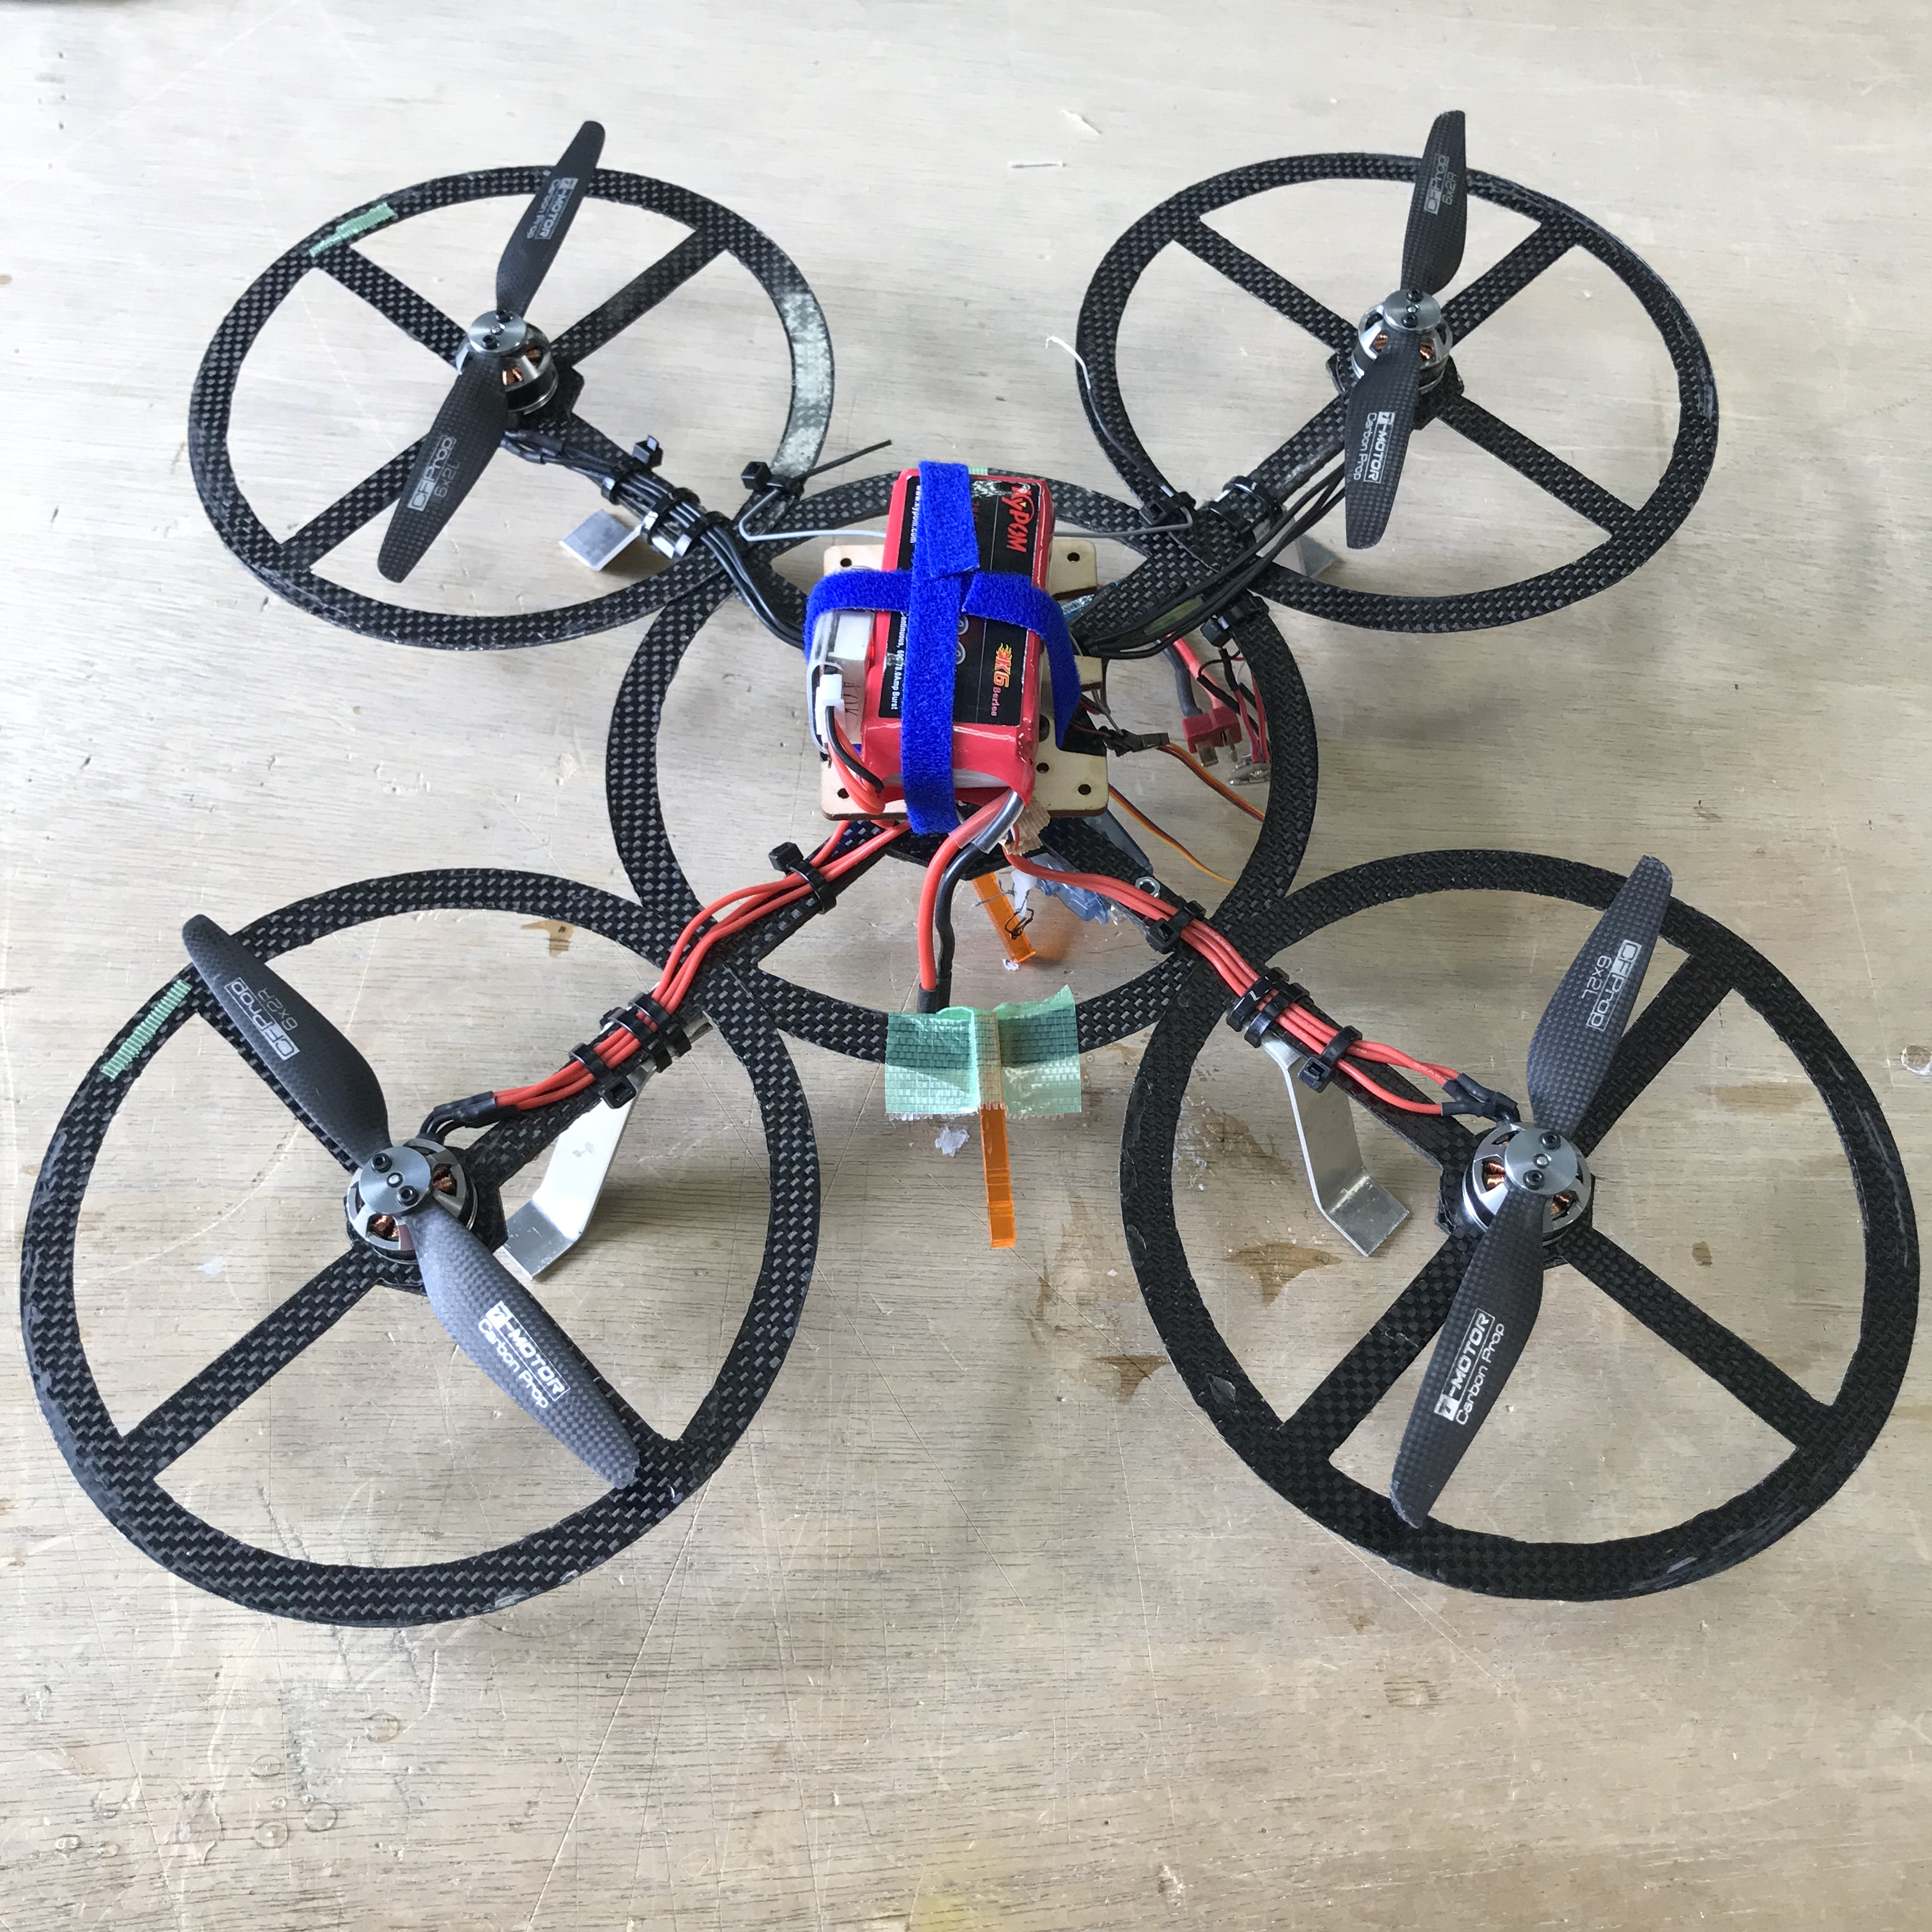
\includegraphics[width=30mm]{img/大会機.jpeg}
    \end{center}
  \caption{飛行ロボコン出場用ロボット}
 \label{fig:ensyu3tex}
\end{figure}

\subsection{研究の目的}
自動制御の課題がいくつかあり,その中に高度制御を利用した自動着陸があり,課題を達成するため高度制御について研究する.


\section{高度制御}

高度センサーで高度を計測して,制御する.センサーの性能を測定した.以下にその結果を示す.

\subsection{超音波センサーの性能確認}
以下に実験手順を示す.


\begin{enumerate}
  \item 距離と出力の確認.
アクリル板を少しずつずらして,距離と出力の関係を確認した.
\begin{figure}[htbp]
  \begin{center}
   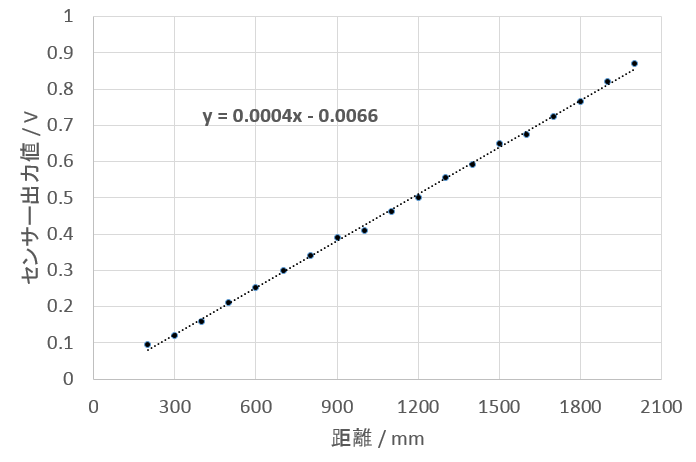
\includegraphics[width=70mm]{img/距離と出力.jpg}
    \end{center}
  \caption{超音波センサーの距離と出力の関係}
 \label{fig:ensyu3tex}
\end{figure}
図3より,距離に応じてセンサーの出力値が比例していることがわかる.
%\end{itemize}
  \item 検知範囲の確認.
%\begin{itemize}
センサーの検知範囲を確認した.
\begin{figure}[htbp]
  \begin{center}
   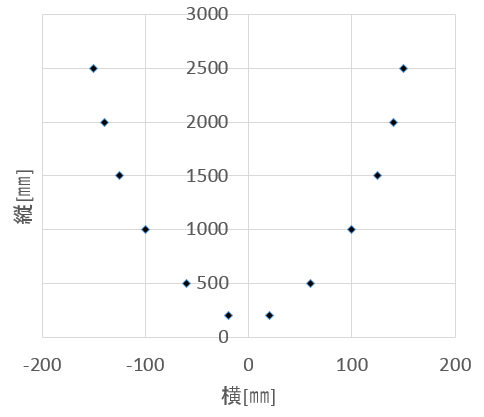
\includegraphics[width=60mm]{img/検知範囲.jpg}
    \end{center}
  \caption{超音波センサーの検知範囲}
 \label{fig:ensyu3tex}
\end{figure}
図4より超音波センサーの音波は広範囲に広がって検知している.
超音波センサーの性能を確認することができた.

\end{enumerate}
\subsection{PID制御}
偏差(目標値と現在値の差)に比例して制御量が増える比例制御(P),偏差がある状態が長時間続くにつれ制御量が増えていく積分制御(I),偏差が急激な変化をするほど制御量が増える微分制御(D)を組み合わせた基本的な制御手法である.
ブロック線図を図5に示す.%\subsubsection{極配置法}
\begin{figure}[htbp]
  \begin{center}
   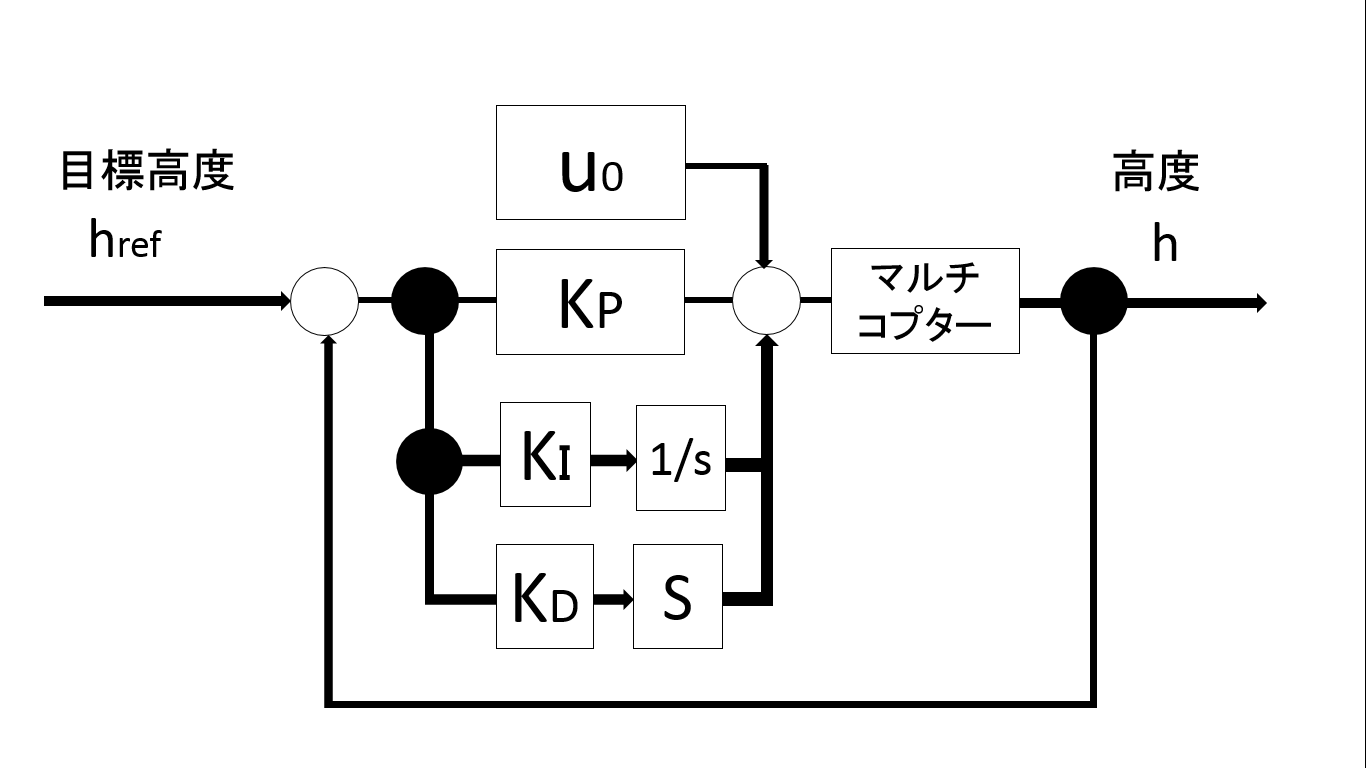
\includegraphics[width=65mm]{img/ブロック図.jpg}
    \end{center}
  \caption{ブロック線図}
 \label{fig:ensyu3tex}
\end{figure}

\section{高度制御のシミュレーション実験}
制御性能をシュミレーションで確認する.

Pythonによって製作された制御シミュレーションCADを用いて,PID制御の比例ゲイン$K_P$,積分ゲイン$K_I$,微分ゲイン$K_D$に値を入れてシミュレーションを模擬実験する.

\section{実験結果}
\begin{enumerate}
  \item 比例制御のみの結果を図6示す.
比例制御だけでは発散して,高度制御ができないことがわかる.
  \item 比例制御と微分制御の実験を行った結果を図7示す.
微分制御を加えたことで,安定するが目標値に一致しないことがわかる.
  \item 積分制御を使った結果を図8示す.


積分制御を加えたことで,目標値に一致していることがわかる.

\begin{figure}[htbp]
  \begin{center}
   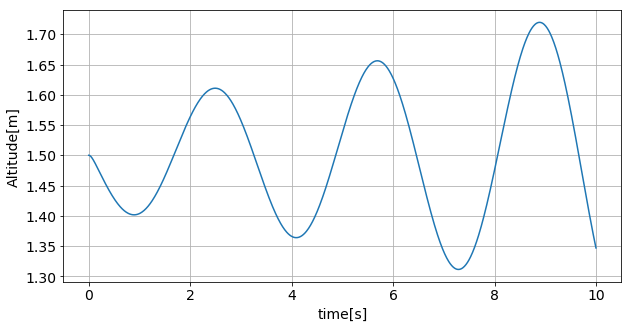
\includegraphics[width=75mm]{img/発散.jpg}
    \end{center}
  \caption{比例制御のみの計算結果}
 \label{fig:ensyu3tex}
\end{figure}

\begin{figure}[htbp]
  \begin{center}
   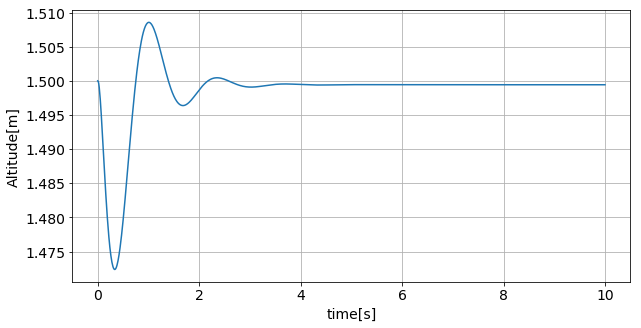
\includegraphics[width=75mm]{img/PD.jpg}
    \end{center}
  \caption{比例制御,微分制御の計算結果}
 \label{fig:ensyu3tex}
\end{figure}

\begin{figure}[htbp]
  \begin{center}
   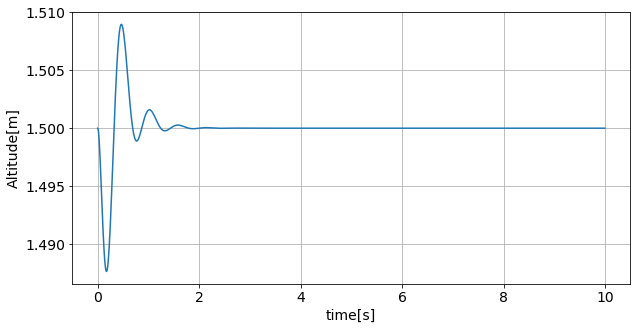
\includegraphics[width=75mm]{img/PIDbest.jpg}
    \end{center}
  \caption{比例制御,微分制御,積分制御の計算結果}
 \label{fig:ensyu3tex}
\end{figure}


\section{おわりに}
高度制御について超音波センサーの性能確認の実験とPID制御を利用したシミュレーション実験を行った.
PID制御をすることにより高度制御を成功した.


しかし制御し始めに少しだけ落ちてしまっているため更に研究が必要である.


加えて,実機での実験を今後実施する.

% 参考文献
\begin{thebibliography}{8}
和栗雄大郎,模型飛行機の科学,養賢堂,2005/07
%\bibitem{ob} 熊谷正朗,状態フィードバックとオブザーバ,www.mech.tohoku-gakuin.ac.jp\slash{}rde\slash{}contents\slash{}course\slash{}controlII\slash{}statefeedback.html,2011\slash{}02\slash{}10
%\bibitem{sei} 明石 一・今井弘之,制御工学演習,共立出版,2014\slash{}04\slash{}15
\end{thebibliography}


\end{document}